% Created by tikzDevice version 0.12.3.1 on 2021-06-16 15:27:59
% !TEX encoding = UTF-8 Unicode
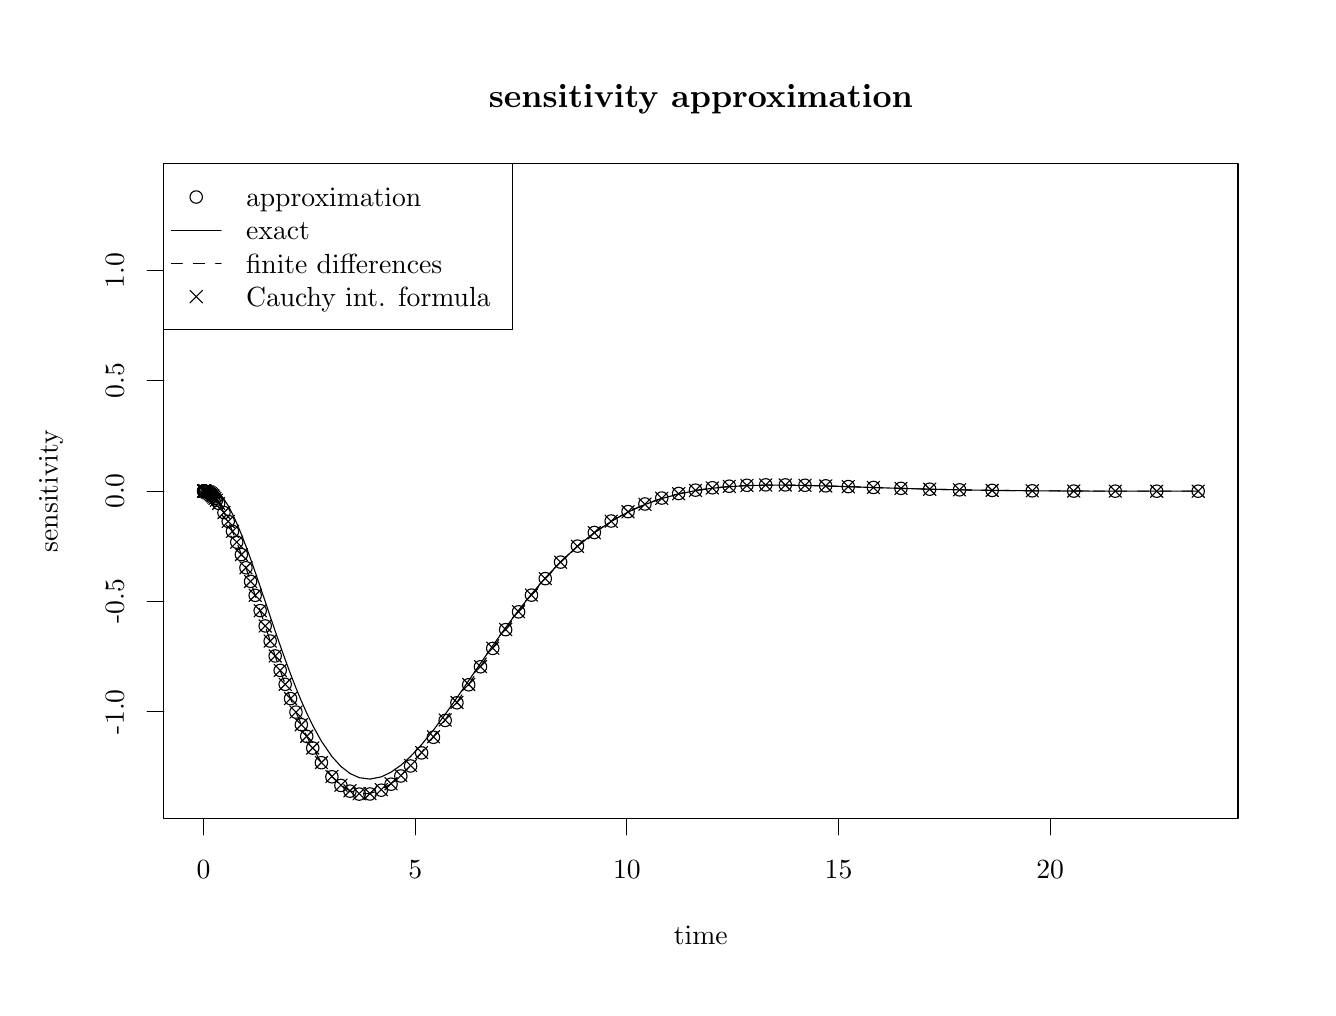
\begin{tikzpicture}[x=1pt,y=1pt]
\definecolor{fillColor}{RGB}{255,255,255}
\path[use as bounding box,fill=fillColor,fill opacity=0.00] (0,0) rectangle (462.53,346.90);
\begin{scope}
\path[clip] ( 49.20, 61.20) rectangle (437.33,297.70);
\definecolor{drawColor}{RGB}{0,0,0}

\path[draw=drawColor,line width= 0.4pt,line join=round,line cap=round] ( 63.58,179.45) circle (  2.25);

\path[draw=drawColor,line width= 0.4pt,line join=round,line cap=round] ( 63.60,179.45) circle (  2.25);

\path[draw=drawColor,line width= 0.4pt,line join=round,line cap=round] ( 63.63,179.45) circle (  2.25);

\path[draw=drawColor,line width= 0.4pt,line join=round,line cap=round] ( 63.66,179.45) circle (  2.25);

\path[draw=drawColor,line width= 0.4pt,line join=round,line cap=round] ( 63.70,179.45) circle (  2.25);

\path[draw=drawColor,line width= 0.4pt,line join=round,line cap=round] ( 63.73,179.44) circle (  2.25);

\path[draw=drawColor,line width= 0.4pt,line join=round,line cap=round] ( 63.76,179.44) circle (  2.25);

\path[draw=drawColor,line width= 0.4pt,line join=round,line cap=round] ( 63.79,179.44) circle (  2.25);

\path[draw=drawColor,line width= 0.4pt,line join=round,line cap=round] ( 63.84,179.44) circle (  2.25);

\path[draw=drawColor,line width= 0.4pt,line join=round,line cap=round] ( 63.91,179.43) circle (  2.25);

\path[draw=drawColor,line width= 0.4pt,line join=round,line cap=round] ( 64.04,179.41) circle (  2.25);

\path[draw=drawColor,line width= 0.4pt,line join=round,line cap=round] ( 64.27,179.37) circle (  2.25);

\path[draw=drawColor,line width= 0.4pt,line join=round,line cap=round] ( 64.77,179.21) circle (  2.25);

\path[draw=drawColor,line width= 0.4pt,line join=round,line cap=round] ( 65.18,179.02) circle (  2.25);

\path[draw=drawColor,line width= 0.4pt,line join=round,line cap=round] ( 65.60,178.78) circle (  2.25);

\path[draw=drawColor,line width= 0.4pt,line join=round,line cap=round] ( 66.02,178.48) circle (  2.25);

\path[draw=drawColor,line width= 0.4pt,line join=round,line cap=round] ( 66.44,178.14) circle (  2.25);

\path[draw=drawColor,line width= 0.4pt,line join=round,line cap=round] ( 66.86,177.74) circle (  2.25);

\path[draw=drawColor,line width= 0.4pt,line join=round,line cap=round] ( 67.28,177.30) circle (  2.25);

\path[draw=drawColor,line width= 0.4pt,line join=round,line cap=round] ( 67.70,176.81) circle (  2.25);

\path[draw=drawColor,line width= 0.4pt,line join=round,line cap=round] ( 68.22,176.14) circle (  2.25);

\path[draw=drawColor,line width= 0.4pt,line join=round,line cap=round] ( 69.00,175.01) circle (  2.25);

\path[draw=drawColor,line width= 0.4pt,line join=round,line cap=round] ( 70.92,171.68) circle (  2.25);

\path[draw=drawColor,line width= 0.4pt,line join=round,line cap=round] ( 72.46,168.49) circle (  2.25);

\path[draw=drawColor,line width= 0.4pt,line join=round,line cap=round] ( 74.01,164.91) circle (  2.25);

\path[draw=drawColor,line width= 0.4pt,line join=round,line cap=round] ( 75.55,161.00) circle (  2.25);

\path[draw=drawColor,line width= 0.4pt,line join=round,line cap=round] ( 77.22,156.49) circle (  2.25);

\path[draw=drawColor,line width= 0.4pt,line join=round,line cap=round] ( 78.88,151.74) circle (  2.25);

\path[draw=drawColor,line width= 0.4pt,line join=round,line cap=round] ( 80.55,146.82) circle (  2.25);

\path[draw=drawColor,line width= 0.4pt,line join=round,line cap=round] ( 82.21,141.78) circle (  2.25);

\path[draw=drawColor,line width= 0.4pt,line join=round,line cap=round] ( 84.02,136.25) circle (  2.25);

\path[draw=drawColor,line width= 0.4pt,line join=round,line cap=round] ( 85.83,130.72) circle (  2.25);

\path[draw=drawColor,line width= 0.4pt,line join=round,line cap=round] ( 87.63,125.25) circle (  2.25);

\path[draw=drawColor,line width= 0.4pt,line join=round,line cap=round] ( 89.44,119.87) circle (  2.25);

\path[draw=drawColor,line width= 0.4pt,line join=round,line cap=round] ( 91.25,114.65) circle (  2.25);

\path[draw=drawColor,line width= 0.4pt,line join=round,line cap=round] ( 93.05,109.62) circle (  2.25);

\path[draw=drawColor,line width= 0.4pt,line join=round,line cap=round] ( 95.00,104.45) circle (  2.25);

\path[draw=drawColor,line width= 0.4pt,line join=round,line cap=round] ( 96.95, 99.58) circle (  2.25);

\path[draw=drawColor,line width= 0.4pt,line join=round,line cap=round] ( 98.89, 95.03) circle (  2.25);

\path[draw=drawColor,line width= 0.4pt,line join=round,line cap=round] (100.84, 90.83) circle (  2.25);

\path[draw=drawColor,line width= 0.4pt,line join=round,line cap=round] (103.01, 86.58) circle (  2.25);

\path[draw=drawColor,line width= 0.4pt,line join=round,line cap=round] (106.14, 81.29) circle (  2.25);

\path[draw=drawColor,line width= 0.4pt,line join=round,line cap=round] (109.94, 76.21) circle (  2.25);

\path[draw=drawColor,line width= 0.4pt,line join=round,line cap=round] (113.19, 73.08) circle (  2.25);

\path[draw=drawColor,line width= 0.4pt,line join=round,line cap=round] (116.45, 71.02) circle (  2.25);

\path[draw=drawColor,line width= 0.4pt,line join=round,line cap=round] (119.81, 69.96) circle (  2.25);

\path[draw=drawColor,line width= 0.4pt,line join=round,line cap=round] (123.68, 69.99) circle (  2.25);

\path[draw=drawColor,line width= 0.4pt,line join=round,line cap=round] (127.77, 71.36) circle (  2.25);

\path[draw=drawColor,line width= 0.4pt,line join=round,line cap=round] (131.31, 73.53) circle (  2.25);

\path[draw=drawColor,line width= 0.4pt,line join=round,line cap=round] (134.84, 76.49) circle (  2.25);

\path[draw=drawColor,line width= 0.4pt,line join=round,line cap=round] (138.37, 80.11) circle (  2.25);

\path[draw=drawColor,line width= 0.4pt,line join=round,line cap=round] (142.35, 84.84) circle (  2.25);

\path[draw=drawColor,line width= 0.4pt,line join=round,line cap=round] (146.61, 90.48) circle (  2.25);

\path[draw=drawColor,line width= 0.4pt,line join=round,line cap=round] (150.86, 96.58) circle (  2.25);

\path[draw=drawColor,line width= 0.4pt,line join=round,line cap=round] (155.11,102.95) circle (  2.25);

\path[draw=drawColor,line width= 0.4pt,line join=round,line cap=round] (159.37,109.45) circle (  2.25);

\path[draw=drawColor,line width= 0.4pt,line join=round,line cap=round] (163.62,115.95) circle (  2.25);

\path[draw=drawColor,line width= 0.4pt,line join=round,line cap=round] (168.05,122.60) circle (  2.25);

\path[draw=drawColor,line width= 0.4pt,line join=round,line cap=round] (172.71,129.37) circle (  2.25);

\path[draw=drawColor,line width= 0.4pt,line join=round,line cap=round] (177.38,135.81) circle (  2.25);

\path[draw=drawColor,line width= 0.4pt,line join=round,line cap=round] (182.04,141.85) circle (  2.25);

\path[draw=drawColor,line width= 0.4pt,line join=round,line cap=round] (187.03,147.81) circle (  2.25);

\path[draw=drawColor,line width= 0.4pt,line join=round,line cap=round] (192.57,153.78) circle (  2.25);

\path[draw=drawColor,line width= 0.4pt,line join=round,line cap=round] (198.66,159.55) circle (  2.25);

\path[draw=drawColor,line width= 0.4pt,line join=round,line cap=round] (204.76,164.48) circle (  2.25);

\path[draw=drawColor,line width= 0.4pt,line join=round,line cap=round] (210.85,168.63) circle (  2.25);

\path[draw=drawColor,line width= 0.4pt,line join=round,line cap=round] (216.94,172.03) circle (  2.25);

\path[draw=drawColor,line width= 0.4pt,line join=round,line cap=round] (223.04,174.78) circle (  2.25);

\path[draw=drawColor,line width= 0.4pt,line join=round,line cap=round] (229.13,176.93) circle (  2.25);

\path[draw=drawColor,line width= 0.4pt,line join=round,line cap=round] (235.23,178.57) circle (  2.25);

\path[draw=drawColor,line width= 0.4pt,line join=round,line cap=round] (241.32,179.78) circle (  2.25);

\path[draw=drawColor,line width= 0.4pt,line join=round,line cap=round] (247.41,180.64) circle (  2.25);

\path[draw=drawColor,line width= 0.4pt,line join=round,line cap=round] (253.51,181.20) circle (  2.25);

\path[draw=drawColor,line width= 0.4pt,line join=round,line cap=round] (259.89,181.54) circle (  2.25);

\path[draw=drawColor,line width= 0.4pt,line join=round,line cap=round] (266.67,181.69) circle (  2.25);

\path[draw=drawColor,line width= 0.4pt,line join=round,line cap=round] (273.77,181.68) circle (  2.25);

\path[draw=drawColor,line width= 0.4pt,line join=round,line cap=round] (280.87,181.55) circle (  2.25);

\path[draw=drawColor,line width= 0.4pt,line join=round,line cap=round] (288.35,181.34) circle (  2.25);

\path[draw=drawColor,line width= 0.4pt,line join=round,line cap=round] (296.52,181.07) circle (  2.25);

\path[draw=drawColor,line width= 0.4pt,line join=round,line cap=round] (305.61,180.75) circle (  2.25);

\path[draw=drawColor,line width= 0.4pt,line join=round,line cap=round] (315.56,180.43) circle (  2.25);

\path[draw=drawColor,line width= 0.4pt,line join=round,line cap=round] (325.94,180.13) circle (  2.25);

\path[draw=drawColor,line width= 0.4pt,line join=round,line cap=round] (336.72,179.89) circle (  2.25);

\path[draw=drawColor,line width= 0.4pt,line join=round,line cap=round] (348.51,179.69) circle (  2.25);

\path[draw=drawColor,line width= 0.4pt,line join=round,line cap=round] (363.00,179.54) circle (  2.25);

\path[draw=drawColor,line width= 0.4pt,line join=round,line cap=round] (377.99,179.45) circle (  2.25);

\path[draw=drawColor,line width= 0.4pt,line join=round,line cap=round] (392.98,179.42) circle (  2.25);

\path[draw=drawColor,line width= 0.4pt,line join=round,line cap=round] (407.96,179.41) circle (  2.25);

\path[draw=drawColor,line width= 0.4pt,line join=round,line cap=round] (422.95,179.41) circle (  2.25);
\end{scope}
\begin{scope}
\path[clip] (  0.00,  0.00) rectangle (462.53,346.90);
\definecolor{drawColor}{RGB}{0,0,0}

\path[draw=drawColor,line width= 0.4pt,line join=round,line cap=round] ( 63.58, 61.20) -- (369.49, 61.20);

\path[draw=drawColor,line width= 0.4pt,line join=round,line cap=round] ( 63.58, 61.20) -- ( 63.58, 55.20);

\path[draw=drawColor,line width= 0.4pt,line join=round,line cap=round] (140.06, 61.20) -- (140.06, 55.20);

\path[draw=drawColor,line width= 0.4pt,line join=round,line cap=round] (216.54, 61.20) -- (216.54, 55.20);

\path[draw=drawColor,line width= 0.4pt,line join=round,line cap=round] (293.02, 61.20) -- (293.02, 55.20);

\path[draw=drawColor,line width= 0.4pt,line join=round,line cap=round] (369.49, 61.20) -- (369.49, 55.20);

\node[text=drawColor,anchor=base,inner sep=0pt, outer sep=0pt, scale=  1.00] at ( 63.58, 39.60) {0};

\node[text=drawColor,anchor=base,inner sep=0pt, outer sep=0pt, scale=  1.00] at (140.06, 39.60) {5};

\node[text=drawColor,anchor=base,inner sep=0pt, outer sep=0pt, scale=  1.00] at (216.54, 39.60) {10};

\node[text=drawColor,anchor=base,inner sep=0pt, outer sep=0pt, scale=  1.00] at (293.02, 39.60) {15};

\node[text=drawColor,anchor=base,inner sep=0pt, outer sep=0pt, scale=  1.00] at (369.49, 39.60) {20};

\path[draw=drawColor,line width= 0.4pt,line join=round,line cap=round] ( 49.20, 99.71) -- ( 49.20,259.19);

\path[draw=drawColor,line width= 0.4pt,line join=round,line cap=round] ( 49.20, 99.71) -- ( 43.20, 99.71);

\path[draw=drawColor,line width= 0.4pt,line join=round,line cap=round] ( 49.20,139.58) -- ( 43.20,139.58);

\path[draw=drawColor,line width= 0.4pt,line join=round,line cap=round] ( 49.20,179.45) -- ( 43.20,179.45);

\path[draw=drawColor,line width= 0.4pt,line join=round,line cap=round] ( 49.20,219.32) -- ( 43.20,219.32);

\path[draw=drawColor,line width= 0.4pt,line join=round,line cap=round] ( 49.20,259.19) -- ( 43.20,259.19);

\node[text=drawColor,rotate= 90.00,anchor=base,inner sep=0pt, outer sep=0pt, scale=  1.00] at ( 34.80, 99.71) {-1.0};

\node[text=drawColor,rotate= 90.00,anchor=base,inner sep=0pt, outer sep=0pt, scale=  1.00] at ( 34.80,139.58) {-0.5};

\node[text=drawColor,rotate= 90.00,anchor=base,inner sep=0pt, outer sep=0pt, scale=  1.00] at ( 34.80,179.45) {0.0};

\node[text=drawColor,rotate= 90.00,anchor=base,inner sep=0pt, outer sep=0pt, scale=  1.00] at ( 34.80,219.32) {0.5};

\node[text=drawColor,rotate= 90.00,anchor=base,inner sep=0pt, outer sep=0pt, scale=  1.00] at ( 34.80,259.19) {1.0};

\path[draw=drawColor,line width= 0.4pt,line join=round,line cap=round] ( 49.20, 61.20) --
	(437.33, 61.20) --
	(437.33,297.70) --
	( 49.20,297.70) --
	( 49.20, 61.20);
\end{scope}
\begin{scope}
\path[clip] (  0.00,  0.00) rectangle (462.53,346.90);
\definecolor{drawColor}{RGB}{0,0,0}

\node[text=drawColor,anchor=base,inner sep=0pt, outer sep=0pt, scale=  1.20] at (243.26,318.16) {\bfseries sensitivity approximation};

\node[text=drawColor,anchor=base,inner sep=0pt, outer sep=0pt, scale=  1.00] at (243.26, 15.60) {time};

\node[text=drawColor,rotate= 90.00,anchor=base,inner sep=0pt, outer sep=0pt, scale=  1.00] at ( 10.80,179.45) {sensitivity};
\end{scope}
\begin{scope}
\path[clip] ( 49.20, 61.20) rectangle (437.33,297.70);
\definecolor{drawColor}{RGB}{0,0,0}

\path[draw=drawColor,line width= 0.4pt,line join=round,line cap=round] ( 63.58,179.45) --
	( 63.60,179.47) --
	( 63.63,179.50) --
	( 63.66,179.52) --
	( 63.70,179.55) --
	( 63.73,179.57) --
	( 63.76,179.60) --
	( 63.79,179.62) --
	( 63.84,179.66) --
	( 63.91,179.71) --
	( 64.04,179.80) --
	( 64.27,179.95) --
	( 64.77,180.19) --
	( 65.18,180.33) --
	( 65.60,180.40) --
	( 66.02,180.41) --
	( 66.44,180.37) --
	( 66.86,180.26) --
	( 67.28,180.10) --
	( 67.70,179.88) --
	( 68.22,179.55) --
	( 69.00,178.88) --
	( 70.92,176.59) --
	( 72.46,174.13) --
	( 74.01,171.18) --
	( 75.55,167.83) --
	( 77.22,163.83) --
	( 78.88,159.51) --
	( 80.55,154.94) --
	( 82.21,150.18) --
	( 84.02,144.89) --
	( 85.83,139.53) --
	( 87.63,134.16) --
	( 89.44,128.84) --
	( 91.25,123.63) --
	( 93.05,118.56) --
	( 95.00,113.30) --
	( 96.95,108.30) --
	( 98.89,103.60) --
	(100.84, 99.22) --
	(103.01, 94.73) --
	(106.14, 89.08) --
	(109.94, 83.53) --
	(113.19, 79.95) --
	(116.45, 77.42) --
	(119.81, 75.88) --
	(123.68, 75.37) --
	(127.77, 76.18) --
	(131.31, 77.87) --
	(134.84, 80.37) --
	(138.37, 83.56) --
	(142.35, 87.85) --
	(146.61, 93.06) --
	(150.86, 98.76) --
	(155.11,104.77) --
	(159.37,110.96) --
	(163.62,117.18) --
	(168.05,123.58) --
	(172.71,130.12) --
	(177.38,136.36) --
	(182.04,142.23) --
	(187.03,148.05) --
	(192.57,153.89) --
	(198.66,159.55) --
	(204.76,164.41) --
	(210.85,168.50) --
	(216.94,171.87) --
	(223.04,174.59) --
	(229.13,176.74) --
	(235.23,178.39) --
	(241.32,179.61) --
	(247.41,180.47) --
	(253.51,181.05) --
	(259.89,181.41) --
	(266.67,181.58) --
	(273.77,181.59) --
	(280.87,181.48) --
	(288.35,181.29) --
	(296.52,181.03) --
	(305.61,180.73) --
	(315.56,180.41) --
	(325.94,180.13) --
	(336.72,179.89) --
	(348.51,179.70) --
	(363.00,179.55) --
	(377.99,179.47) --
	(392.98,179.43) --
	(407.96,179.41) --
	(422.95,179.42);

\path[draw=drawColor,line width= 0.4pt,dash pattern=on 4pt off 4pt ,line join=round,line cap=round] ( 63.58,179.45) --
	( 63.60,179.45) --
	( 63.63,179.45) --
	( 63.66,179.45) --
	( 63.70,179.45) --
	( 63.73,179.44) --
	( 63.76,179.44) --
	( 63.79,179.44) --
	( 63.84,179.44) --
	( 63.91,179.43) --
	( 64.04,179.41) --
	( 64.27,179.37) --
	( 64.77,179.21) --
	( 65.18,179.02) --
	( 65.60,178.78) --
	( 66.02,178.48) --
	( 66.44,178.14) --
	( 66.86,177.74) --
	( 67.28,177.30) --
	( 67.70,176.81) --
	( 68.22,176.14) --
	( 69.00,175.00) --
	( 70.92,171.68) --
	( 72.46,168.48) --
	( 74.01,164.89) --
	( 75.55,160.99) --
	( 77.22,156.48) --
	( 78.88,151.73) --
	( 80.55,146.80) --
	( 82.21,141.77) --
	( 84.02,136.24) --
	( 85.83,130.71) --
	( 87.63,125.24) --
	( 89.44,119.87) --
	( 91.25,114.65) --
	( 93.05,109.63) --
	( 95.00,104.46) --
	( 96.95, 99.59) --
	( 98.89, 95.04) --
	(100.84, 90.85) --
	(103.01, 86.61) --
	(106.14, 81.34) --
	(109.94, 76.31) --
	(113.19, 73.19) --
	(116.45, 71.15) --
	(119.81, 70.10) --
	(123.68, 70.16) --
	(127.77, 71.55) --
	(131.31, 73.72) --
	(134.84, 76.67) --
	(138.37, 80.28) --
	(142.35, 85.00) --
	(146.61, 90.64) --
	(150.86, 96.73) --
	(155.11,103.08) --
	(159.37,109.56) --
	(163.62,116.05) --
	(168.05,122.68) --
	(172.71,129.43) --
	(177.38,135.85) --
	(182.04,141.86) --
	(187.03,147.81) --
	(192.57,153.76) --
	(198.66,159.50) --
	(204.76,164.42) --
	(210.85,168.55) --
	(216.94,171.95) --
	(223.04,174.68) --
	(229.13,176.83) --
	(235.23,178.48) --
	(241.32,179.69) --
	(247.41,180.55) --
	(253.51,181.12) --
	(259.89,181.47) --
	(266.67,181.63) --
	(273.77,181.63) --
	(280.87,181.51) --
	(288.35,181.31) --
	(296.52,181.05) --
	(305.61,180.74) --
	(315.56,180.42) --
	(325.94,180.13) --
	(336.72,179.90) --
	(348.51,179.70) --
	(363.00,179.55) --
	(377.99,179.46) --
	(392.98,179.43) --
	(407.96,179.41) --
	(422.95,179.42);

\path[draw=drawColor,line width= 0.4pt,line join=round,line cap=round] ( 61.33,177.20) -- ( 65.83,181.70);

\path[draw=drawColor,line width= 0.4pt,line join=round,line cap=round] ( 61.33,181.70) -- ( 65.83,177.20);

\path[draw=drawColor,line width= 0.4pt,line join=round,line cap=round] ( 61.35,177.20) -- ( 65.85,181.70);

\path[draw=drawColor,line width= 0.4pt,line join=round,line cap=round] ( 61.35,181.70) -- ( 65.85,177.20);

\path[draw=drawColor,line width= 0.4pt,line join=round,line cap=round] ( 61.38,177.20) -- ( 65.88,181.70);

\path[draw=drawColor,line width= 0.4pt,line join=round,line cap=round] ( 61.38,181.70) -- ( 65.88,177.20);

\path[draw=drawColor,line width= 0.4pt,line join=round,line cap=round] ( 61.41,177.20) -- ( 65.91,181.70);

\path[draw=drawColor,line width= 0.4pt,line join=round,line cap=round] ( 61.41,181.70) -- ( 65.91,177.20);

\path[draw=drawColor,line width= 0.4pt,line join=round,line cap=round] ( 61.45,177.20) -- ( 65.95,181.70);

\path[draw=drawColor,line width= 0.4pt,line join=round,line cap=round] ( 61.45,181.70) -- ( 65.95,177.20);

\path[draw=drawColor,line width= 0.4pt,line join=round,line cap=round] ( 61.48,177.19) -- ( 65.98,181.69);

\path[draw=drawColor,line width= 0.4pt,line join=round,line cap=round] ( 61.48,181.69) -- ( 65.98,177.19);

\path[draw=drawColor,line width= 0.4pt,line join=round,line cap=round] ( 61.51,177.19) -- ( 66.01,181.69);

\path[draw=drawColor,line width= 0.4pt,line join=round,line cap=round] ( 61.51,181.69) -- ( 66.01,177.19);

\path[draw=drawColor,line width= 0.4pt,line join=round,line cap=round] ( 61.54,177.19) -- ( 66.04,181.69);

\path[draw=drawColor,line width= 0.4pt,line join=round,line cap=round] ( 61.54,181.69) -- ( 66.04,177.19);

\path[draw=drawColor,line width= 0.4pt,line join=round,line cap=round] ( 61.59,177.19) -- ( 66.09,181.69);

\path[draw=drawColor,line width= 0.4pt,line join=round,line cap=round] ( 61.59,181.69) -- ( 66.09,177.19);

\path[draw=drawColor,line width= 0.4pt,line join=round,line cap=round] ( 61.66,177.18) -- ( 66.16,181.68);

\path[draw=drawColor,line width= 0.4pt,line join=round,line cap=round] ( 61.66,181.68) -- ( 66.16,177.18);

\path[draw=drawColor,line width= 0.4pt,line join=round,line cap=round] ( 61.79,177.16) -- ( 66.29,181.66);

\path[draw=drawColor,line width= 0.4pt,line join=round,line cap=round] ( 61.79,181.66) -- ( 66.29,177.16);

\path[draw=drawColor,line width= 0.4pt,line join=round,line cap=round] ( 62.02,177.12) -- ( 66.52,181.62);

\path[draw=drawColor,line width= 0.4pt,line join=round,line cap=round] ( 62.02,181.62) -- ( 66.52,177.12);

\path[draw=drawColor,line width= 0.4pt,line join=round,line cap=round] ( 62.52,176.96) -- ( 67.02,181.46);

\path[draw=drawColor,line width= 0.4pt,line join=round,line cap=round] ( 62.52,181.46) -- ( 67.02,176.96);

\path[draw=drawColor,line width= 0.4pt,line join=round,line cap=round] ( 62.93,176.77) -- ( 67.43,181.27);

\path[draw=drawColor,line width= 0.4pt,line join=round,line cap=round] ( 62.93,181.27) -- ( 67.43,176.77);

\path[draw=drawColor,line width= 0.4pt,line join=round,line cap=round] ( 63.35,176.53) -- ( 67.85,181.03);

\path[draw=drawColor,line width= 0.4pt,line join=round,line cap=round] ( 63.35,181.03) -- ( 67.85,176.53);

\path[draw=drawColor,line width= 0.4pt,line join=round,line cap=round] ( 63.77,176.23) -- ( 68.27,180.73);

\path[draw=drawColor,line width= 0.4pt,line join=round,line cap=round] ( 63.77,180.73) -- ( 68.27,176.23);

\path[draw=drawColor,line width= 0.4pt,line join=round,line cap=round] ( 64.19,175.89) -- ( 68.69,180.39);

\path[draw=drawColor,line width= 0.4pt,line join=round,line cap=round] ( 64.19,180.39) -- ( 68.69,175.89);

\path[draw=drawColor,line width= 0.4pt,line join=round,line cap=round] ( 64.61,175.49) -- ( 69.11,179.99);

\path[draw=drawColor,line width= 0.4pt,line join=round,line cap=round] ( 64.61,179.99) -- ( 69.11,175.49);

\path[draw=drawColor,line width= 0.4pt,line join=round,line cap=round] ( 65.03,175.05) -- ( 69.53,179.55);

\path[draw=drawColor,line width= 0.4pt,line join=round,line cap=round] ( 65.03,179.55) -- ( 69.53,175.05);

\path[draw=drawColor,line width= 0.4pt,line join=round,line cap=round] ( 65.45,174.56) -- ( 69.95,179.06);

\path[draw=drawColor,line width= 0.4pt,line join=round,line cap=round] ( 65.45,179.06) -- ( 69.95,174.56);

\path[draw=drawColor,line width= 0.4pt,line join=round,line cap=round] ( 65.97,173.89) -- ( 70.47,178.39);

\path[draw=drawColor,line width= 0.4pt,line join=round,line cap=round] ( 65.97,178.39) -- ( 70.47,173.89);

\path[draw=drawColor,line width= 0.4pt,line join=round,line cap=round] ( 66.75,172.75) -- ( 71.25,177.25);

\path[draw=drawColor,line width= 0.4pt,line join=round,line cap=round] ( 66.75,177.25) -- ( 71.25,172.75);

\path[draw=drawColor,line width= 0.4pt,line join=round,line cap=round] ( 68.67,169.43) -- ( 73.17,173.93);

\path[draw=drawColor,line width= 0.4pt,line join=round,line cap=round] ( 68.67,173.93) -- ( 73.17,169.43);

\path[draw=drawColor,line width= 0.4pt,line join=round,line cap=round] ( 70.21,166.23) -- ( 74.71,170.73);

\path[draw=drawColor,line width= 0.4pt,line join=round,line cap=round] ( 70.21,170.73) -- ( 74.71,166.23);

\path[draw=drawColor,line width= 0.4pt,line join=round,line cap=round] ( 71.76,162.64) -- ( 76.26,167.14);

\path[draw=drawColor,line width= 0.4pt,line join=round,line cap=round] ( 71.76,167.14) -- ( 76.26,162.64);

\path[draw=drawColor,line width= 0.4pt,line join=round,line cap=round] ( 73.30,158.74) -- ( 77.80,163.24);

\path[draw=drawColor,line width= 0.4pt,line join=round,line cap=round] ( 73.30,163.24) -- ( 77.80,158.74);

\path[draw=drawColor,line width= 0.4pt,line join=round,line cap=round] ( 74.97,154.23) -- ( 79.47,158.73);

\path[draw=drawColor,line width= 0.4pt,line join=round,line cap=round] ( 74.97,158.73) -- ( 79.47,154.23);

\path[draw=drawColor,line width= 0.4pt,line join=round,line cap=round] ( 76.63,149.48) -- ( 81.13,153.98);

\path[draw=drawColor,line width= 0.4pt,line join=round,line cap=round] ( 76.63,153.98) -- ( 81.13,149.48);

\path[draw=drawColor,line width= 0.4pt,line join=round,line cap=round] ( 78.30,144.55) -- ( 82.80,149.05);

\path[draw=drawColor,line width= 0.4pt,line join=round,line cap=round] ( 78.30,149.05) -- ( 82.80,144.55);

\path[draw=drawColor,line width= 0.4pt,line join=round,line cap=round] ( 79.96,139.52) -- ( 84.46,144.02);

\path[draw=drawColor,line width= 0.4pt,line join=round,line cap=round] ( 79.96,144.02) -- ( 84.46,139.52);

\path[draw=drawColor,line width= 0.4pt,line join=round,line cap=round] ( 81.77,133.99) -- ( 86.27,138.49);

\path[draw=drawColor,line width= 0.4pt,line join=round,line cap=round] ( 81.77,138.49) -- ( 86.27,133.99);

\path[draw=drawColor,line width= 0.4pt,line join=round,line cap=round] ( 83.58,128.46) -- ( 88.08,132.96);

\path[draw=drawColor,line width= 0.4pt,line join=round,line cap=round] ( 83.58,132.96) -- ( 88.08,128.46);

\path[draw=drawColor,line width= 0.4pt,line join=round,line cap=round] ( 85.38,122.99) -- ( 89.88,127.49);

\path[draw=drawColor,line width= 0.4pt,line join=round,line cap=round] ( 85.38,127.49) -- ( 89.88,122.99);

\path[draw=drawColor,line width= 0.4pt,line join=round,line cap=round] ( 87.19,117.62) -- ( 91.69,122.12);

\path[draw=drawColor,line width= 0.4pt,line join=round,line cap=round] ( 87.19,122.12) -- ( 91.69,117.62);

\path[draw=drawColor,line width= 0.4pt,line join=round,line cap=round] ( 89.00,112.40) -- ( 93.50,116.90);

\path[draw=drawColor,line width= 0.4pt,line join=round,line cap=round] ( 89.00,116.90) -- ( 93.50,112.40);

\path[draw=drawColor,line width= 0.4pt,line join=round,line cap=round] ( 90.80,107.38) -- ( 95.30,111.88);

\path[draw=drawColor,line width= 0.4pt,line join=round,line cap=round] ( 90.80,111.88) -- ( 95.30,107.38);

\path[draw=drawColor,line width= 0.4pt,line join=round,line cap=round] ( 92.75,102.21) -- ( 97.25,106.71);

\path[draw=drawColor,line width= 0.4pt,line join=round,line cap=round] ( 92.75,106.71) -- ( 97.25,102.21);

\path[draw=drawColor,line width= 0.4pt,line join=round,line cap=round] ( 94.70, 97.34) -- ( 99.20,101.84);

\path[draw=drawColor,line width= 0.4pt,line join=round,line cap=round] ( 94.70,101.84) -- ( 99.20, 97.34);

\path[draw=drawColor,line width= 0.4pt,line join=round,line cap=round] ( 96.64, 92.79) -- (101.14, 97.29);

\path[draw=drawColor,line width= 0.4pt,line join=round,line cap=round] ( 96.64, 97.29) -- (101.14, 92.79);

\path[draw=drawColor,line width= 0.4pt,line join=round,line cap=round] ( 98.59, 88.60) -- (103.09, 93.10);

\path[draw=drawColor,line width= 0.4pt,line join=round,line cap=round] ( 98.59, 93.10) -- (103.09, 88.60);

\path[draw=drawColor,line width= 0.4pt,line join=round,line cap=round] (100.76, 84.36) -- (105.26, 88.86);

\path[draw=drawColor,line width= 0.4pt,line join=round,line cap=round] (100.76, 88.86) -- (105.26, 84.36);

\path[draw=drawColor,line width= 0.4pt,line join=round,line cap=round] (103.89, 79.09) -- (108.39, 83.59);

\path[draw=drawColor,line width= 0.4pt,line join=round,line cap=round] (103.89, 83.59) -- (108.39, 79.09);

\path[draw=drawColor,line width= 0.4pt,line join=round,line cap=round] (107.69, 74.06) -- (112.19, 78.56);

\path[draw=drawColor,line width= 0.4pt,line join=round,line cap=round] (107.69, 78.56) -- (112.19, 74.06);

\path[draw=drawColor,line width= 0.4pt,line join=round,line cap=round] (110.94, 70.94) -- (115.44, 75.44);

\path[draw=drawColor,line width= 0.4pt,line join=round,line cap=round] (110.94, 75.44) -- (115.44, 70.94);

\path[draw=drawColor,line width= 0.4pt,line join=round,line cap=round] (114.20, 68.90) -- (118.70, 73.40);

\path[draw=drawColor,line width= 0.4pt,line join=round,line cap=round] (114.20, 73.40) -- (118.70, 68.90);

\path[draw=drawColor,line width= 0.4pt,line join=round,line cap=round] (117.56, 67.85) -- (122.06, 72.35);

\path[draw=drawColor,line width= 0.4pt,line join=round,line cap=round] (117.56, 72.35) -- (122.06, 67.85);

\path[draw=drawColor,line width= 0.4pt,line join=round,line cap=round] (121.43, 67.91) -- (125.93, 72.41);

\path[draw=drawColor,line width= 0.4pt,line join=round,line cap=round] (121.43, 72.41) -- (125.93, 67.91);

\path[draw=drawColor,line width= 0.4pt,line join=round,line cap=round] (125.52, 69.30) -- (130.02, 73.80);

\path[draw=drawColor,line width= 0.4pt,line join=round,line cap=round] (125.52, 73.80) -- (130.02, 69.30);

\path[draw=drawColor,line width= 0.4pt,line join=round,line cap=round] (129.06, 71.47) -- (133.56, 75.97);

\path[draw=drawColor,line width= 0.4pt,line join=round,line cap=round] (129.06, 75.97) -- (133.56, 71.47);

\path[draw=drawColor,line width= 0.4pt,line join=round,line cap=round] (132.59, 74.42) -- (137.09, 78.92);

\path[draw=drawColor,line width= 0.4pt,line join=round,line cap=round] (132.59, 78.92) -- (137.09, 74.42);

\path[draw=drawColor,line width= 0.4pt,line join=round,line cap=round] (136.12, 78.03) -- (140.62, 82.53);

\path[draw=drawColor,line width= 0.4pt,line join=round,line cap=round] (136.12, 82.53) -- (140.62, 78.03);

\path[draw=drawColor,line width= 0.4pt,line join=round,line cap=round] (140.10, 82.75) -- (144.60, 87.25);

\path[draw=drawColor,line width= 0.4pt,line join=round,line cap=round] (140.10, 87.25) -- (144.60, 82.75);

\path[draw=drawColor,line width= 0.4pt,line join=round,line cap=round] (144.36, 88.39) -- (148.86, 92.89);

\path[draw=drawColor,line width= 0.4pt,line join=round,line cap=round] (144.36, 92.89) -- (148.86, 88.39);

\path[draw=drawColor,line width= 0.4pt,line join=round,line cap=round] (148.61, 94.48) -- (153.11, 98.98);

\path[draw=drawColor,line width= 0.4pt,line join=round,line cap=round] (148.61, 98.98) -- (153.11, 94.48);

\path[draw=drawColor,line width= 0.4pt,line join=round,line cap=round] (152.86,100.83) -- (157.36,105.33);

\path[draw=drawColor,line width= 0.4pt,line join=round,line cap=round] (152.86,105.33) -- (157.36,100.83);

\path[draw=drawColor,line width= 0.4pt,line join=round,line cap=round] (157.12,107.31) -- (161.62,111.81);

\path[draw=drawColor,line width= 0.4pt,line join=round,line cap=round] (157.12,111.81) -- (161.62,107.31);

\path[draw=drawColor,line width= 0.4pt,line join=round,line cap=round] (161.37,113.80) -- (165.87,118.30);

\path[draw=drawColor,line width= 0.4pt,line join=round,line cap=round] (161.37,118.30) -- (165.87,113.80);

\path[draw=drawColor,line width= 0.4pt,line join=round,line cap=round] (165.80,120.43) -- (170.30,124.93);

\path[draw=drawColor,line width= 0.4pt,line join=round,line cap=round] (165.80,124.93) -- (170.30,120.43);

\path[draw=drawColor,line width= 0.4pt,line join=round,line cap=round] (170.46,127.18) -- (174.96,131.68);

\path[draw=drawColor,line width= 0.4pt,line join=round,line cap=round] (170.46,131.68) -- (174.96,127.18);

\path[draw=drawColor,line width= 0.4pt,line join=round,line cap=round] (175.13,133.60) -- (179.63,138.10);

\path[draw=drawColor,line width= 0.4pt,line join=round,line cap=round] (175.13,138.10) -- (179.63,133.60);

\path[draw=drawColor,line width= 0.4pt,line join=round,line cap=round] (179.79,139.61) -- (184.29,144.11);

\path[draw=drawColor,line width= 0.4pt,line join=round,line cap=round] (179.79,144.11) -- (184.29,139.61);

\path[draw=drawColor,line width= 0.4pt,line join=round,line cap=round] (184.78,145.56) -- (189.28,150.06);

\path[draw=drawColor,line width= 0.4pt,line join=round,line cap=round] (184.78,150.06) -- (189.28,145.56);

\path[draw=drawColor,line width= 0.4pt,line join=round,line cap=round] (190.32,151.51) -- (194.82,156.01);

\path[draw=drawColor,line width= 0.4pt,line join=round,line cap=round] (190.32,156.01) -- (194.82,151.51);

\path[draw=drawColor,line width= 0.4pt,line join=round,line cap=round] (196.41,157.25) -- (200.91,161.75);

\path[draw=drawColor,line width= 0.4pt,line join=round,line cap=round] (196.41,161.75) -- (200.91,157.25);

\path[draw=drawColor,line width= 0.4pt,line join=round,line cap=round] (202.51,162.17) -- (207.01,166.67);

\path[draw=drawColor,line width= 0.4pt,line join=round,line cap=round] (202.51,166.67) -- (207.01,162.17);

\path[draw=drawColor,line width= 0.4pt,line join=round,line cap=round] (208.60,166.30) -- (213.10,170.80);

\path[draw=drawColor,line width= 0.4pt,line join=round,line cap=round] (208.60,170.80) -- (213.10,166.30);

\path[draw=drawColor,line width= 0.4pt,line join=round,line cap=round] (214.69,169.70) -- (219.19,174.20);

\path[draw=drawColor,line width= 0.4pt,line join=round,line cap=round] (214.69,174.20) -- (219.19,169.70);

\path[draw=drawColor,line width= 0.4pt,line join=round,line cap=round] (220.79,172.43) -- (225.29,176.93);

\path[draw=drawColor,line width= 0.4pt,line join=round,line cap=round] (220.79,176.93) -- (225.29,172.43);

\path[draw=drawColor,line width= 0.4pt,line join=round,line cap=round] (226.88,174.58) -- (231.38,179.08);

\path[draw=drawColor,line width= 0.4pt,line join=round,line cap=round] (226.88,179.08) -- (231.38,174.58);

\path[draw=drawColor,line width= 0.4pt,line join=round,line cap=round] (232.98,176.23) -- (237.48,180.73);

\path[draw=drawColor,line width= 0.4pt,line join=round,line cap=round] (232.98,180.73) -- (237.48,176.23);

\path[draw=drawColor,line width= 0.4pt,line join=round,line cap=round] (239.07,177.44) -- (243.57,181.94);

\path[draw=drawColor,line width= 0.4pt,line join=round,line cap=round] (239.07,181.94) -- (243.57,177.44);

\path[draw=drawColor,line width= 0.4pt,line join=round,line cap=round] (245.16,178.30) -- (249.66,182.80);

\path[draw=drawColor,line width= 0.4pt,line join=round,line cap=round] (245.16,182.80) -- (249.66,178.30);

\path[draw=drawColor,line width= 0.4pt,line join=round,line cap=round] (251.26,178.87) -- (255.76,183.37);

\path[draw=drawColor,line width= 0.4pt,line join=round,line cap=round] (251.26,183.37) -- (255.76,178.87);

\path[draw=drawColor,line width= 0.4pt,line join=round,line cap=round] (257.64,179.22) -- (262.14,183.72);

\path[draw=drawColor,line width= 0.4pt,line join=round,line cap=round] (257.64,183.72) -- (262.14,179.22);

\path[draw=drawColor,line width= 0.4pt,line join=round,line cap=round] (264.42,179.38) -- (268.92,183.88);

\path[draw=drawColor,line width= 0.4pt,line join=round,line cap=round] (264.42,183.88) -- (268.92,179.38);

\path[draw=drawColor,line width= 0.4pt,line join=round,line cap=round] (271.52,179.38) -- (276.02,183.88);

\path[draw=drawColor,line width= 0.4pt,line join=round,line cap=round] (271.52,183.88) -- (276.02,179.38);

\path[draw=drawColor,line width= 0.4pt,line join=round,line cap=round] (278.62,179.26) -- (283.12,183.76);

\path[draw=drawColor,line width= 0.4pt,line join=round,line cap=round] (278.62,183.76) -- (283.12,179.26);

\path[draw=drawColor,line width= 0.4pt,line join=round,line cap=round] (286.10,179.06) -- (290.60,183.56);

\path[draw=drawColor,line width= 0.4pt,line join=round,line cap=round] (286.10,183.56) -- (290.60,179.06);

\path[draw=drawColor,line width= 0.4pt,line join=round,line cap=round] (294.27,178.80) -- (298.77,183.30);

\path[draw=drawColor,line width= 0.4pt,line join=round,line cap=round] (294.27,183.30) -- (298.77,178.80);

\path[draw=drawColor,line width= 0.4pt,line join=round,line cap=round] (303.36,178.49) -- (307.86,182.99);

\path[draw=drawColor,line width= 0.4pt,line join=round,line cap=round] (303.36,182.99) -- (307.86,178.49);

\path[draw=drawColor,line width= 0.4pt,line join=round,line cap=round] (313.31,178.17) -- (317.81,182.67);

\path[draw=drawColor,line width= 0.4pt,line join=round,line cap=round] (313.31,182.67) -- (317.81,178.17);

\path[draw=drawColor,line width= 0.4pt,line join=round,line cap=round] (323.69,177.88) -- (328.19,182.38);

\path[draw=drawColor,line width= 0.4pt,line join=round,line cap=round] (323.69,182.38) -- (328.19,177.88);

\path[draw=drawColor,line width= 0.4pt,line join=round,line cap=round] (334.47,177.65) -- (338.97,182.15);

\path[draw=drawColor,line width= 0.4pt,line join=round,line cap=round] (334.47,182.15) -- (338.97,177.65);

\path[draw=drawColor,line width= 0.4pt,line join=round,line cap=round] (346.26,177.45) -- (350.76,181.95);

\path[draw=drawColor,line width= 0.4pt,line join=round,line cap=round] (346.26,181.95) -- (350.76,177.45);

\path[draw=drawColor,line width= 0.4pt,line join=round,line cap=round] (360.75,177.30) -- (365.25,181.80);

\path[draw=drawColor,line width= 0.4pt,line join=round,line cap=round] (360.75,181.80) -- (365.25,177.30);

\path[draw=drawColor,line width= 0.4pt,line join=round,line cap=round] (375.74,177.21) -- (380.24,181.71);

\path[draw=drawColor,line width= 0.4pt,line join=round,line cap=round] (375.74,181.71) -- (380.24,177.21);

\path[draw=drawColor,line width= 0.4pt,line join=round,line cap=round] (390.73,177.18) -- (395.23,181.68);

\path[draw=drawColor,line width= 0.4pt,line join=round,line cap=round] (390.73,181.68) -- (395.23,177.18);

\path[draw=drawColor,line width= 0.4pt,line join=round,line cap=round] (405.71,177.17) -- (410.21,181.67);

\path[draw=drawColor,line width= 0.4pt,line join=round,line cap=round] (405.71,181.67) -- (410.21,177.17);

\path[draw=drawColor,line width= 0.4pt,line join=round,line cap=round] (420.70,177.17) -- (425.20,181.67);

\path[draw=drawColor,line width= 0.4pt,line join=round,line cap=round] (420.70,181.67) -- (425.20,177.17);
\definecolor{fillColor}{RGB}{255,255,255}

\path[draw=drawColor,line width= 0.4pt,line join=round,line cap=round,fill=fillColor] ( 49.20,297.70) rectangle (175.18,237.70);

\path[draw=drawColor,line width= 0.4pt,line join=round,line cap=round] ( 51.90,273.70) -- ( 69.90,273.70);

\path[draw=drawColor,line width= 0.4pt,dash pattern=on 4pt off 4pt ,line join=round,line cap=round] ( 51.90,261.70) -- ( 69.90,261.70);

\path[draw=drawColor,line width= 0.4pt,line join=round,line cap=round] ( 60.90,285.70) circle (  2.25);

\path[draw=drawColor,line width= 0.4pt,line join=round,line cap=round] ( 58.65,247.45) -- ( 63.15,251.95);

\path[draw=drawColor,line width= 0.4pt,line join=round,line cap=round] ( 58.65,251.95) -- ( 63.15,247.45);

\node[text=drawColor,anchor=base west,inner sep=0pt, outer sep=0pt, scale=  1.00] at ( 78.90,282.25) {approximation};

\node[text=drawColor,anchor=base west,inner sep=0pt, outer sep=0pt, scale=  1.00] at ( 78.90,270.25) {exact};

\node[text=drawColor,anchor=base west,inner sep=0pt, outer sep=0pt, scale=  1.00] at ( 78.90,258.25) {finite differences};

\node[text=drawColor,anchor=base west,inner sep=0pt, outer sep=0pt, scale=  1.00] at ( 78.90,246.25) {Cauchy int. formula};
\end{scope}
\end{tikzpicture}
